\documentclass[11pt, a4paper]{article}
\usepackage{polski}
\usepackage[utf8]{inputenc}
\usepackage[T1]{fontenc}
\usepackage[export]{adjustbox}
\usepackage{graphicx}
\usepackage{amsmath} 
\usepackage{listings}
\usepackage{color}
\usepackage{marvosym}
\usepackage{geometry}
\usepackage{enumerate}
\usepackage{float}
\usepackage{booktabs}
\usepackage{multirow}
\usepackage{titlesec}
\usepackage{hyperref}
\usepackage{tabularx}
\usepackage{amssymb}
\usepackage{algorithm}
\usepackage[noend]{algpseudocode}

\geometry{margin=1.2in}
\usepackage[final]{pdfpages}

\newcommand{\fbi}{\leavevmode{\parindent=1em\indent}}

\definecolor{dkgreen}{rgb}{0,0.6,0}
\definecolor{gray}{rgb}{0.5,0.5,0.5}
\definecolor{mauve}{rgb}{0.58,0,0.82}

\floatname{algorithm}{Pseudokod}

\lstset{
	frame=tblr,
	language=Matlab,
	aboveskip=3mm,
	belowskip=3mm,
	showstringspaces=false,
	columns=flexible,
	basicstyle={\small\ttfamily},
	numbers=left,
	numberstyle=\tiny\color{gray},
	keywordstyle=\color{blue},
	commentstyle=\color{dkgreen},
	stringstyle=\color{mauve},
	breaklines=true,
	mathescape=false,
	breakatwhitespace=true,
	tabsize=3,
	inputencoding=utf8,
	extendedchars=true,
	literate=
	{ą}{{\k{a}}}1
	{Ą}{{\k{A}}}1
	{ę}{{\k{e}}}1
	{Ę}{{\k{E}}}1
	{ó}{{\'o}}1
	{Ó}{{\'O}}1
	{ś}{{\'s}}1
	{Ś}{{\'S}}1
	{ł}{{\l{}}}1
	{Ł}{{\L{}}}1
	{ż}{{\.z}}1
	{Ż}{{\.Z}}1
	{ź}{{\'z}}1
	{Ź}{{\'Z}}1
	{ć}{{\'c}}1
	{Ć}{{\'C}}1
	{ń}{{\'n}}1
	{Ń}{{\'N}}1
}

\renewcommand\lstlistingname{Listing}

\titleclass{\subsubsubsection}{straight}[\subsection]
\newcounter{subsubsubsection}[subsubsection]
\renewcommand\thesubsubsubsection{\thesubsubsection.\arabic{subsubsubsection}}
\renewcommand\theparagraph{\thesubsubsubsection.\arabic{paragraph}}

\titleformat{\subsubsubsection}
  {\normalfont\normalsize\bfseries}{\thesubsubsubsection}{1em}{}
\titlespacing*{\subsubsubsection}
{0pt}{3.25ex plus 1ex minus .2ex}{1.5ex plus .2ex}

\makeatletter
\renewcommand\paragraph{\@startsection{paragraph}{5}{\z@}
  {3.25ex \@plus1ex \@minus.2ex}
  {-0em}
  {\normalfont\normalsize\bfseries}}
\renewcommand\subparagraph{\@startsection{subparagraph}{6}{\parindent}
  {3.25ex \@plus1ex \@minus .2ex}
  {-1em}
  {\normalfont\normalsize\bfseries}}
\def\toclevel@subsubsubsection{4}
\def\toclevel@paragraph{5}
\def\toclevel@paragraph{6}
\def\l@subsubsubsection{\@dottedtocline{4}{7em}{4em}}
\def\l@paragraph{\@dottedtocline{5}{10em}{5em}}
\def\l@subparagraph{\@dottedtocline{6}{14em}{6em}}
\makeatother

\setcounter{secnumdepth}{4}
\setcounter{tocdepth}{4}

\hypersetup{pageanchor=false}

\setlength\parindent{3pt}

\renewcommand{\labelenumi}{\alph{enumi}.} 

\date{\today}


\begin{document}

\begin{titlepage}

\newcommand{\HRule}{\rule{\linewidth}{0.5mm}} 
\center 

\textsc{\LARGE Politechnika Wrocławska}\\[1.5cm] 
\textsc{\Large Inteligencja Obliczeniowa i jej zastosowania}\\[0.5cm] 
\HRule \\[0.5cm]
{ \huge \bfseries Ćwiczenie 2 \\*
	Metody redukcji wymiarowości \\*
	Nieujemna faktoryzacja macierzy \\i dekompozycje tensorów}\\[0.5cm] 
\HRule \\[1.6cm]
 
\begin{minipage}{0.4\textwidth}
\begin{flushleft} \large
\emph{Autorzy:}\\
Paweł  \textsc{Andziul} 200648 \\
Robert  \textsc{Chojnacki} 200685 \\
Marcin  \textsc{Słowiński} 200638 \\
\end{flushleft}
\end{minipage}
~
\begin{minipage}{0.4\textwidth}
\begin{flushright} \large
\emph{Prowadzący:} \\
dr hab. inż. Rafał \textsc{Zdunek}
\end{flushright}
\end{minipage}\\[4cm]

\vfill 
{\large 12 czerwca 2017}\\[3cm] 

\end{titlepage}

\tableofcontents

\newpage
\section{Zadanie 1}
\paragraph{}
Wygenerować faktory $A = [a_{ij}] \in R^{I x J}_{+}$ i $X = [x_{jt}] \in R^{J x T}_{+}$, gdzie $a_{ij} = max(0,\check{a}_{ij})$ i $x_{jt} = max(0,\check{x}_{jt})$ oraz $\check{a}_{ij},\check{x}_{jt}\sim N(0,1)$ (rozkład normalny). Wygeneruj syntetyczne obserwacje Y=AX dla I = 100, T = 1000, J = 10. Stosując wybrane algorytmy NMF (ALS, MUE, HALS) wyznacz estymowane faktory \^{A} i \^{X} oraz unormowany błąd residualny w funkcji iteracji naprzemiennych. Oceń jakość estymacji stosując miary MSE (ang. Mean-Squarred Error) lub SIR (ang. Signal-to-Interference Ratio).

\subsection{Algorytm ALS}
\paragraph{}
Algorytm ALS polega na N-krotnym powtórzeniu pętli, której zadaniem jest obliczenie tensorów A oraz X.
Wynik obliczenia jednego tensora wpływa na wynik drugiego, co dla kolejnych iteracji zmniejsza różnice między obrazem właściwym a zredukowanym. Algorytm bazuje na wzorach \ref{eq:als1} oraz \ref{eq:als2}.	

\begin{equation}\label{eq:als1}
\nabla_A D(Y|AX) = (AX - Y)X^T = 0 \Rightarrow AXX^T = YX^T \Rightarrow A = YX^T(XX^T)^{-1}
\end{equation}

\begin{equation}\label{eq:als2}
\nabla_X D(Y|AX) = A^T(AX - Y) = 0 \Rightarrow A^TAX = A^TY \Rightarrow X = (A^TA)^{-1}A^TY
\end{equation}

\fbi
Otrzymane tensory po każdej z iteracji przemnażane są przez siebie otrzymując obraz zredukowany, który następnie jest przyrównywany do oryginału oznaczonego jako Y.

\subsection{Algorytm MUE}
\paragraph{}
Algorytm MUE działa podobnie do algorytmu ALS. Zmieniają się w nim wzory odpowiadające za poszczególne tensory.

\begin{equation}\label{eq:mue1}
a_{ij} = a_{ij}\frac{[YX^T]_{ij}}{[AXX^T]_{ij}}
\end{equation}
\begin{equation}\label{eq:mue2}
x_{jt} = x_{jt}\frac{[A^TY]_{jt}}{[A^TAX]_{jt}}
\end{equation}

\fbi
Zaletą algorytmu MUE jest niski koszt obliczeniowy. Niestety, jest on obarczony kosztem w postaci powolnej zbieżności, co oznacza konieczność wykonania większej ilości obliczeń, które mogą zanegować jego zalety.

\subsection{Algorytm HALS}
\paragraph{}
Algorytm HALS od algorytmu ALS różni się iterowaniem osobno po wierszach i kolumnach.

\begin{equation}\label{eq:hals1}
a_j = [a_j + \dfrac{[YX^T]_{*j} - A[XX^T]_{*j}}{[XX^T]_{jj}}]_+
\end{equation}
\begin{equation}\label{eq:hals2}
x_j = [x_j + \dfrac{[A^TY]_{j*} - [A^TA]_{j*}X}{[A^TA]_{jj}}]_+
\end{equation}

\fbi
Algorytm ten charakteryzuje się najmniejszym błędem residualnym osiąganym już przy niskiej ilości iteracji.

\subsection{Realizacja}
\paragraph{}
Na poniższych listingach zamieszczono praktyczną implementację algorytmów w środowisku MATLAB.

\lstinputlisting[label=lst:zad1main,caption=Skrypt wywołujący realizacje w środowisku MATLAB,firstline=1,lastline=200]{./assets/skrypt_zad1.m}

\newpage
\lstinputlisting[label=lst:zad1als,caption=Algorytm ALS,firstline=1,lastline=200]{./assets/skrypt_zad1_nmf_als.m}

\lstinputlisting[label=lst:zad1mue,caption=Algorytm MUE,firstline=1,lastline=200]{./assets/skrypt_zad1_nmf_mue.m}

\lstinputlisting[label=lst:zad1hals,caption=Algorytm HALS,firstline=1,lastline=200]{./assets/skrypt_zad1_nmf_hals.m}

\subsection{Wyniki}
\paragraph{}
Na ilustracji \ref{fig:wykres_zad1} zamieszczono graficzne porównanie przebiegu optymalizacji kolejno algorytmami ALS, MUE oraz HALS.

\begin{figure}[H]
	\centering
	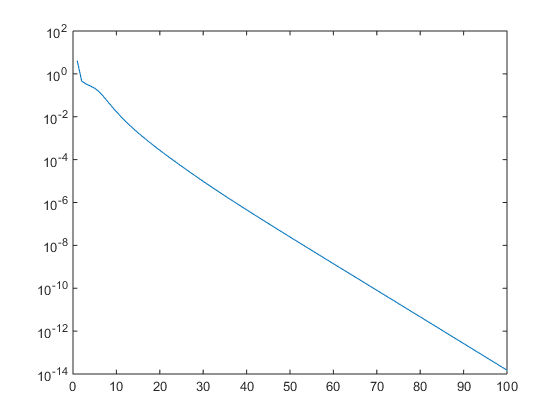
\includegraphics[width=0.95\textwidth]{./assets/wykres_zad1.png}
	\caption{Wykres ilustrujący przebieg optymalizacji ALS, MUE oraz HALS}
	\label{fig:wykres_zad1}
\end{figure}

\begin{figure}[H]
	\centering
	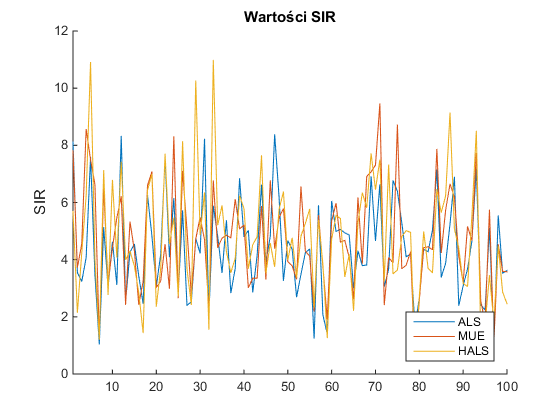
\includegraphics[width=0.6\textwidth]{./assets/wykres_zad1_sir.png}
	\caption{Wykres SIR}
	\label{fig:wykres_zad1_sir}
\end{figure}


\section{Zadanie 2}
\paragraph{}
Wygenerować faktory 
$U^(1) = [u^{(1)}_{i_1j}] \in R_+^{I_1xJ}$,
 $U^(2) = [u^{(2)}_{i_2j}] \in R_+^{I_2xJ}$,
  $U^(3) = [u^{(3)}_{i_3j}] \in R_+^{I_3xJ}$,
  gdzie 
  $[u^{(1)}_{i_1j}] = max(0, \check{u}^{(1)}_{i_1j})$,
  $[u^{(2)}_{i_2j}] = max(0, \check{u}^{(2)}_{i_2j})$,
  $[u^{(3)}_{i_3j}] = max(0, \check{u}^{(3)}_{i_3j})$
  oraz
  $\check{u}^{(1)}_{i_1j}$,
  $\check{u}^{(2)}_{i_2j}$,
  $\check{u}^{(3)}_{i_3j}$
  $\sim N(0,1)$ (rozkład normalny). 
  Wygeneruj syntetyczne obserwacje Y dla 
  $I_1$ = 10, 
  $I_2$ = 20, 
  $I_3$ = 30, 
  $J$ = 5. 
  Stosując wybrane algorytmy NTF (np. ALS) wyznacz estymowane faktory $\check{U}^{(1)}, \check{U}^{(2)}, \check{U}^{(3)}$ oraz unormowany błąd residualny w funkcji iteracji naprzemiennych. Oceń jakość estymacji stosując miary MSE (ang. Mean-Squared Error) lub SIR (ang. Signal-to-Interference Ratio).

\section{Zadanie 3}
\paragraph{}
Obrazy twarzy z bazy ORL (lub podobnej) przedstaw za pomocą tensora $Y \in R^{I_1xI_2xI_3}$, gdzie $I_3$ jest liczbą obrazów. Rozdziel obrazy na zbiory trenujący i testujący według odpowiedniej zasady, np, 5-folds CV i utwórz odpowiednie tensory trenujący $Y_r$ i testujący $Y_t$. Tensor trenujący poddaj dekompozycji CP (np. algorytmem ALS) oraz HOSVD dla J = 4, 10, 20, 30. Pogrupować obrazy stosując metodę k-średnich dla faktora $\widehat{U}^{(3)}$. Badania przeprowadzić dla różnej liczby grup. Porównać dokładność grupowania z metodą PCA (z poprzedniego ćwiczenia). Następnie dokonaj projekcji obrazów z tensora $Y_t$ na podprzestrzeń cech generowaną faktorami otrzymanymi z $Y_r$. Dokonaj klasyfikacji obrazów w przestrzeni cech w $\widehat{U}^{(3)}$ za pomocą klasyfikatora k-NN. Porównać efekty klasyfikacji różnymi metodami (np. PCA, CP, HOSVD).

\subsection{Opis metody}
\paragraph{}
HOSVD jest szczególnym przypadkiem modelu dekompozycji Tuckera. Kolumny każdej z macierzy czynnikowych (faktorów) są wzajemnie ortogonalne, a tensor rdzeniowy $\mathcal {G}$ nie jest superdiagonalny. Dokonujemy kolejno matrycyzacji względem n-tego modu. 

\subsection{Algorytm}
\paragraph{}
Wejściem algorytmu HO-SVD są: tensor danych $Y \in R^{I_1xI_2xI_3}$ oraz rzędy faktoryzacji $J = [J_1, ..., J_N]$, natomiast wyjściem: estymowane wektory $U^{(n)}$ oraz tensor rdzeniowy $\mathcal {G}$.



\begin{algorithm}
	\caption{Algorytm HO-SVD}
	\label{algorytmHosvd}
	\begin{algorithmic}[1]
		\For {\textit{n} = 1, ..., \textit{N}}
		\State $Y_{(n)} \gets $ \text{unfolding($\mathcal {Y}$, n) $\in R^{I_{n}\times \prod _{{p\neq n}}I_{p}}$}
		\State $U_{(n)} \gets $ \text{eigs($ Y_{(n)}(Y_{(n)})^T, J_n$)}
		\EndFor
		\State {Wyznacz tensor $\mathcal {G}$}
	\end{algorithmic}
\end{algorithm}

\subsection{Realizacja}
\paragraph{}
Na kolejnych listingach zamieszczono implementację w środowisku MATLAB. Listing \ref{lst:zad3main} stanowi podstawowy potok przetwarzania od wczytania danych po wyświetlenie wyników pomiarów. Na listingu \ref{lst:zad3hosvd} zamieszczono implementację metody HOSVD. W celu przeprowadzenia klasyfikacji kNN dokonano podziału zbioru wejściowego przy pomocy \textit{cvpartition} 5-folds (podzielono 80 zdjęć na dwa zbiory składające się odpowiednio z 64 i 16 obrazów).

\lstinputlisting[label=lst:zad3main,caption=Podstawowy skrypt z realizacją w środowisku MATLAB,firstline=1,lastline=200]{./assets/skrypt_zad3.m}

\lstinputlisting[label=lst:zad3hosvd,caption=Funkcja realizująca algorytm HOSVD,firstline=1,lastline=200]{./assets/skrypt_zad3_hosvd.m}

\newpage
\subsection{Wyniki}
\paragraph{}
W niniejszym punkcie zamieszczono wyniki dla dekompozycji z wykorzystaniem metody HOSVD. Badaniu poddano 80 obrazów twarzy (ilustracja \ref{fig:twarze_org}) z bazy Uniwersytetu Cambridge \cite{test7}.

\begin{figure}[H]
	\centering
	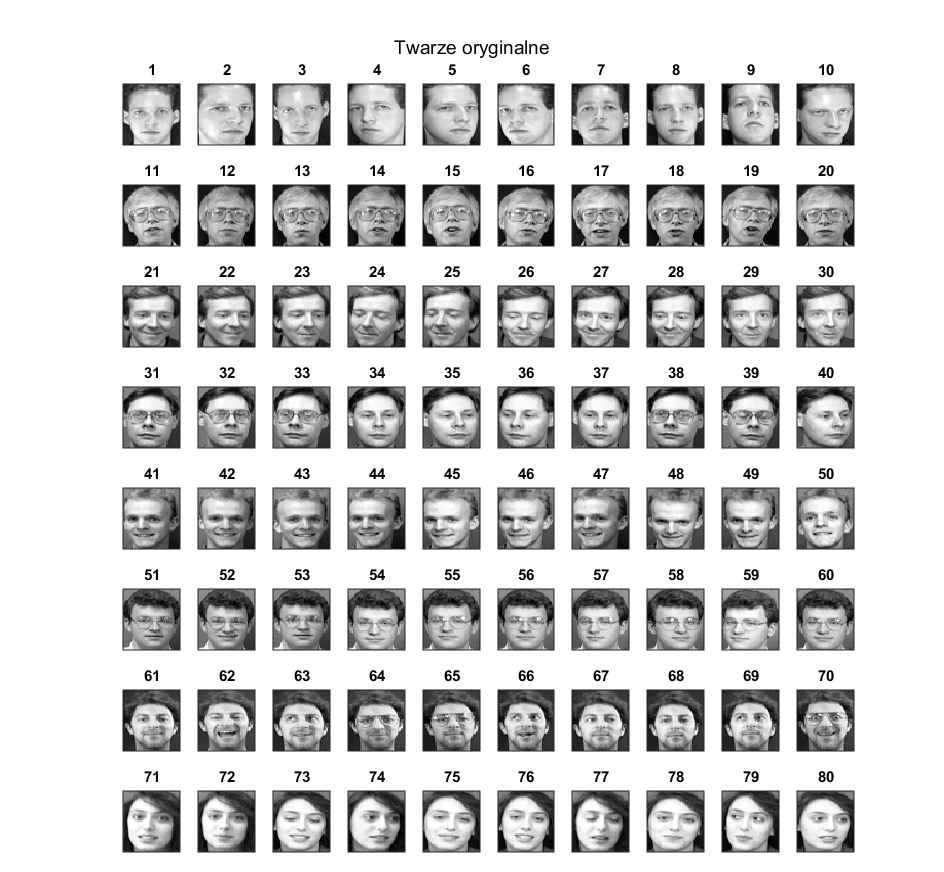
\includegraphics[width=1\textwidth]{./assets/twarze_org.png}
	\caption{Twarze wykorzystane podczas testów}
	\label{fig:twarze_org}
\end{figure}

\newpage
Ilustracja \ref{fig:rezultat_HOSVD_j4} przedstawia wynik grupowania metodą k-średnich dla J=4 oraz liczby grup równej liczbie osób wynoszącej 8.

\begin{figure}[H]
	\centering
	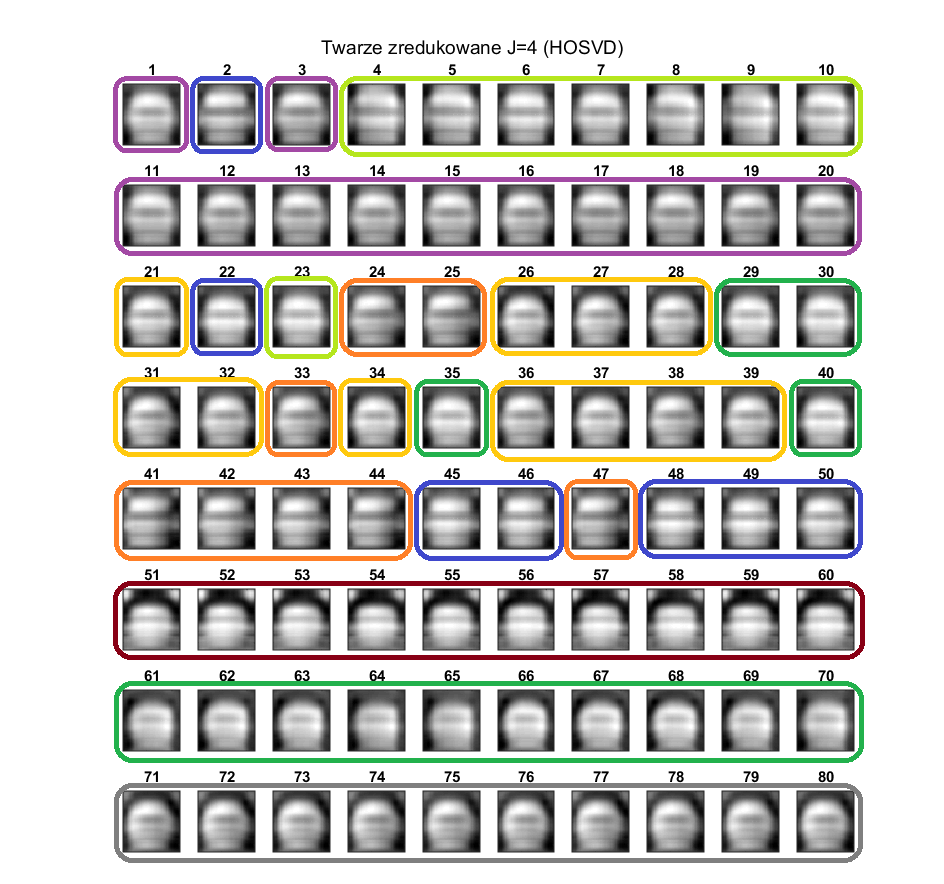
\includegraphics[width=1\textwidth]{./assets/rezultat_HOSVD_j4.png}
	\caption{Twarze zredukowane J=4 (HOSVD)}
	\label{fig:rezultat_HOSVD_j4}
\end{figure}

\newpage
Rysunek \ref{fig:rezultat_HOSVD_j10} przedstawia wynik grupowania metodą k-średnich dla J=10 oraz liczby grup równej liczbie osób wynoszącej 8.

\begin{figure}[H]
	\centering
	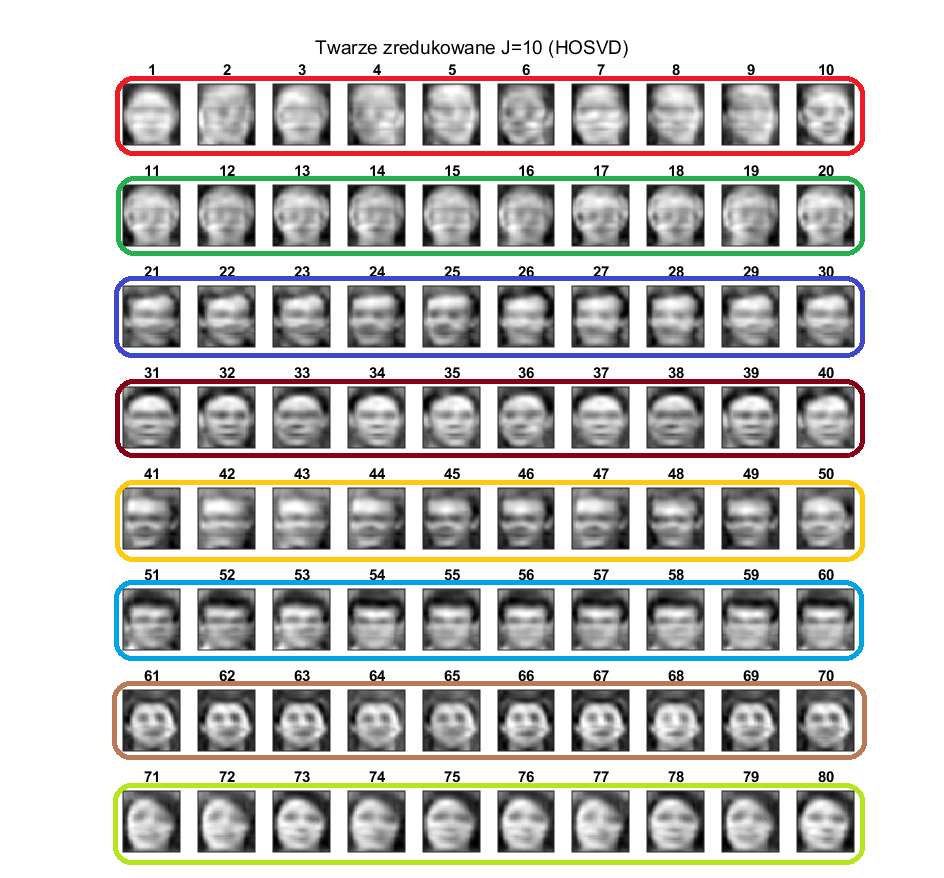
\includegraphics[width=1\textwidth]{./assets/rezultat_HOSVD_j10.png}
	\caption{Twarze zredukowane J=10 (HOSVD)}
	\label{fig:rezultat_HOSVD_j10}
\end{figure}

\newpage
Na ilustracji \ref{fig:rezultat_HOSVD_j20} przedstawiono wynik grupowania metodą k-średnich dla J=20 oraz liczby grup równej liczbie osób wynoszącej 8.

\begin{figure}[H]
	\centering
	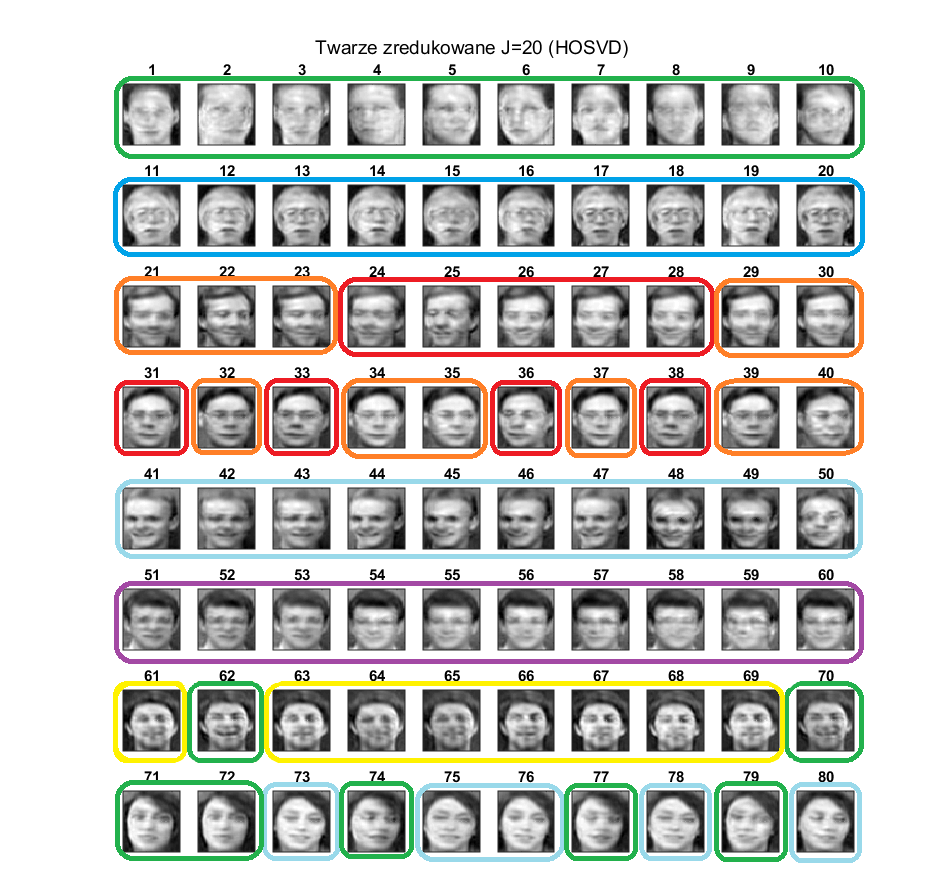
\includegraphics[width=1\textwidth]{./assets/rezultat_HOSVD_j20.png}
	\caption{Twarze zredukowane J=20 (HOSVD)}
	\label{fig:rezultat_HOSVD_j20}
\end{figure}

\newpage
Na rysunku \ref{fig:rezultat_HOSVD_j30} przedstawiono wynik grupowania metodą k-średnich dla J=30 oraz liczby grup równej liczbie osób wynoszącej 8.

\begin{figure}[H]
	\centering
	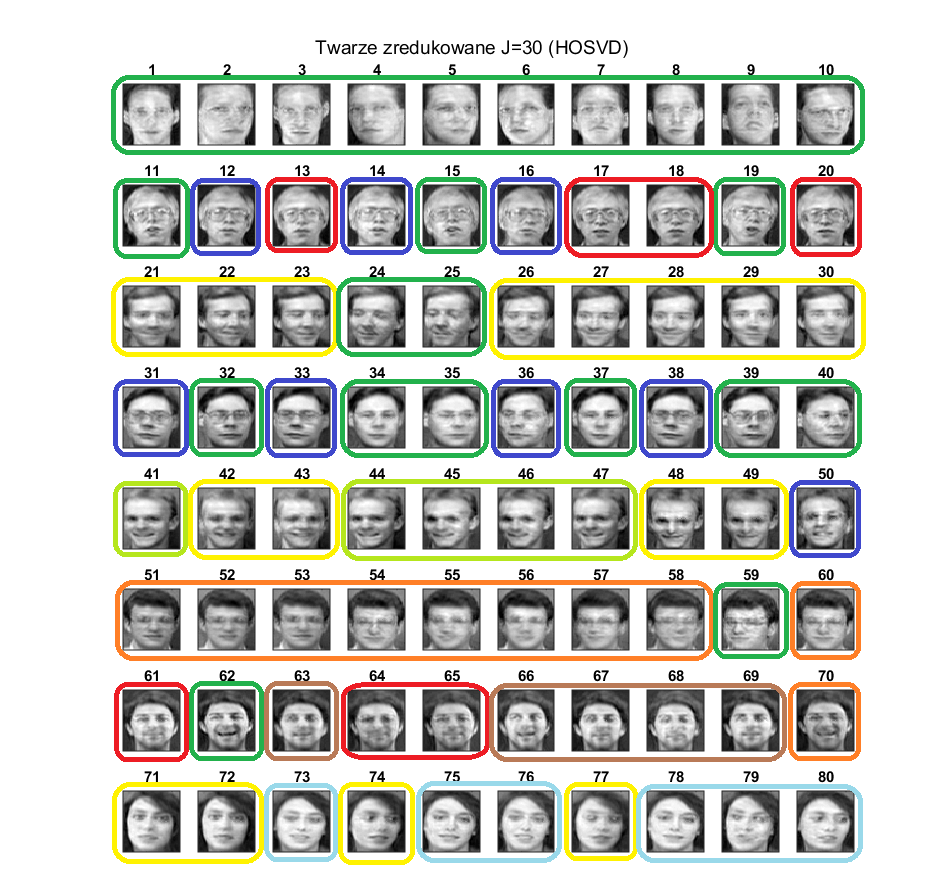
\includegraphics[width=1\textwidth]{./assets/rezultat_HOSVD_j30.png}
	\caption{Twarze zredukowane J=30 (HOSVD)}
	\label{fig:rezultat_HOSVD_j30}
\end{figure}

\fbi
W tabeli \ref{tab:wynikiKmeans} zamieszczono otrzymane wartości metryk. Dla algorytmu k-średnich zostały policzone Acc (dokładność) oraz Rand's index.

\begin{table}[H]
	\centering
	\caption{Otrzymane metryki dla różnych wartości parametru J (k-średnich)}
	\begin{tabular}{|c|c|c|c|c|}
		\hline 
		 & 4 & 10 & 20 & 30 \\ 
		\hline
		Acc (dokładność) & 76,25 & 100 & 80,00 & 63,75 \\
		\hline
		Rand's index & 92,56 & 100 & 93,04 & 84,56 \\
		\hline
	\end{tabular}
	\label{tab:wynikiKmeans}
\end{table}

\fbi
Jak możemy zauważyć metoda k-średnich daje najlepsze rezultaty dla J=10, zarówno mniej jak i więcej szczegółów w obrazie negatywnie wpływa na rezultat grupowania. W przypadku metody najbliższych sąsiadów jest inaczej -- tutaj im bardziej szczegółowy obraz otrzyma ta metoda na wejściu tym lepsze będą rezultaty. Trzeba również pamiętać, że metoda k-średnich nie wymaga zbioru treningowego i uczącego.

W tabeli \ref{tab:wynikiKnn} zamieszczono metryki dla klasyfikacji metodą najbliższych sąsiadów. Zostały policzone dokładność (Acc) oraz Rand's index dla klasyfikacji w przestrzeni cech $\widehat{U}^{(3)}$ przy pomocy metody najbliższych sąsiadów.

\begin{table}[H]
	\centering
	\caption{Otrzymane metryki dla różnych wartości parametru J (k-najbliższych sąsiadów)}
	\begin{tabular}{|c|c|c|c|c|}
		\hline 
		& 4 & 10 & 20 & 30 \\ 
		\hline
		Acc (dokładność) & 81,25 & 93,75 & 100 & 100 \\
		\hline
		Rand's index & 94,17 & 97,50 & 100 & 100 \\
		\hline
	\end{tabular}
	\label{tab:wynikiKnn}
\end{table}

Natomiast zależności czasowe przedstawiono w tabeli \ref{tab:wynikiCzas}. Grupowanie przeprowadzono dla ilości grup równej liczbie osób aby móc jednoznacznie zinterpretować wyniki. Na ilustracji \ref{fig:wykres_zad3_czas} zamieszczono graficzne porównanie.

\begin{table}[H]
	\centering
	\caption{Czas przetwarzania [ms] w zależności od parametru J}
	\begin{tabular}{|c|c|c|c|c|}
		\hline 
		& 4 & 10 & 20 & 30 \\ 
		\hline
		HOSVD & 12,54 & 14,09 & 11,80 & 13,58 \\
		\hline
		grupowanie k-średnich & 8,25 & 9,81 & 11,15 & 15,22 \\
		\hline
		klasyfikacja k-NN & 14,17 & 13,61 & 13,62 & 14,21 \\
		\hline
	\end{tabular}
	\label{tab:wynikiCzas}
\end{table}

\begin{figure}[H]
	\centering
	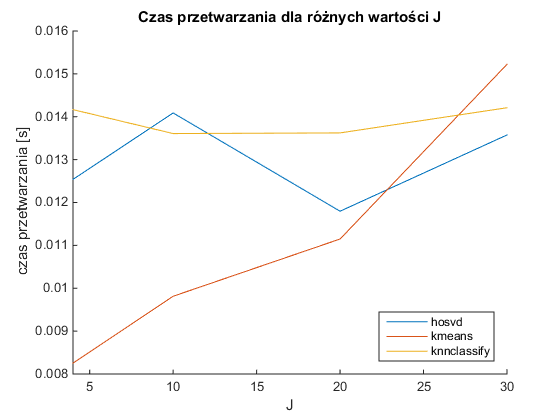
\includegraphics[width=0.85\textwidth]{./assets/wykres_zad3_czas.png}
	\caption{Czas przetwarzania w zależności od wartości J}
	\label{fig:wykres_zad3_czas}
\end{figure}


\section{Podsumowanie}
\paragraph{}
Podczas prac nad zadaniami zapoznano się z metodami redukcji wymiarowości przy pomocy nieujemnej faktoryzacji macierzy i dekompozycji tensorów.


\newpage
\begin{thebibliography}{40}

\bibitem{test1}
Dokumentacja środowiska MATLAB,
\url{https://www.mathworks.com/}

\bibitem{test2}
Zdunek, Rafał, ,,Nieujemna faktoryzacja macierzy i tensorów : zastosowanie do klasyfikacji i przetwarzania sygnałów'', Oficyna Wydawnicza Politechniki Wrocławskiej, 2014

\bibitem{test3}
\url{http://www.sandia.gov/~tgkolda/TensorToolbox/index-2.6.html}

\bibitem{test4}
\url{http://www.esat.kuleuven.be/sista/tensorlab/}

\bibitem{test5}
\url{http://www.bsp.brain.riken.jp/TDALAB/}

\bibitem{test6}
\url{http://www.bsp.brain.riken.jp/~phan/}

\bibitem{test7}
\url{http://www.cl.cam.ac.uk/research/dtg/attarchive/facedatabase.html}

\end{thebibliography}

\end{document}
